% Options for packages loaded elsewhere
\PassOptionsToPackage{unicode}{hyperref}
\PassOptionsToPackage{hyphens}{url}
%
\documentclass[
  10pt,
  ignorenonframetext,
  twocolumn]{beamer}
\usepackage{pgfpages}
\setbeamertemplate{caption}[numbered]
\setbeamertemplate{caption label separator}{: }
\setbeamercolor{caption name}{fg=normal text.fg}
\beamertemplatenavigationsymbolsempty
% Prevent slide breaks in the middle of a paragraph
\widowpenalties 1 10000
\raggedbottom
\setbeamertemplate{part page}{
  \centering
  \begin{beamercolorbox}[sep=16pt,center]{part title}
    \usebeamerfont{part title}\insertpart\par
  \end{beamercolorbox}
}
\setbeamertemplate{section page}{
  \centering
  \begin{beamercolorbox}[sep=12pt,center]{part title}
    \usebeamerfont{section title}\insertsection\par
  \end{beamercolorbox}
}
\setbeamertemplate{subsection page}{
  \centering
  \begin{beamercolorbox}[sep=8pt,center]{part title}
    \usebeamerfont{subsection title}\insertsubsection\par
  \end{beamercolorbox}
}
\AtBeginPart{
  \frame{\partpage}
}
\AtBeginSection{
  \ifbibliography
  \else
    \frame{\sectionpage}
  \fi
}
\AtBeginSubsection{
  \frame{\subsectionpage}
}
\usepackage{amsmath,amssymb}
\usepackage{lmodern}
\usepackage{iftex}
\ifPDFTeX
  \usepackage[T1]{fontenc}
  \usepackage[utf8]{inputenc}
  \usepackage{textcomp} % provide euro and other symbols
\else % if luatex or xetex
  \usepackage{unicode-math}
  \defaultfontfeatures{Scale=MatchLowercase}
  \defaultfontfeatures[\rmfamily]{Ligatures=TeX,Scale=1}
  \setmainfont[]{Baskerville}
\fi
\usetheme[]{Singapore}
\usefonttheme{structurebold}
\usefonttheme{serif} % use mainfont rather than sansfont for slide text
% Use upquote if available, for straight quotes in verbatim environments
\IfFileExists{upquote.sty}{\usepackage{upquote}}{}
\IfFileExists{microtype.sty}{% use microtype if available
  \usepackage[]{microtype}
  \UseMicrotypeSet[protrusion]{basicmath} % disable protrusion for tt fonts
}{}
\makeatletter
\@ifundefined{KOMAClassName}{% if non-KOMA class
  \IfFileExists{parskip.sty}{%
    \usepackage{parskip}
  }{% else
    \setlength{\parindent}{0pt}
    \setlength{\parskip}{6pt plus 2pt minus 1pt}}
}{% if KOMA class
  \KOMAoptions{parskip=half}}
\makeatother
\usepackage{xcolor}
\newif\ifbibliography
\usepackage{longtable,booktabs,array}
\usepackage{calc} % for calculating minipage widths
\usepackage{caption}
% Make caption package work with longtable
\makeatletter
\def\fnum@table{\tablename~\thetable}
\makeatother
\setlength{\emergencystretch}{3em} % prevent overfull lines
\providecommand{\tightlist}{%
  \setlength{\itemsep}{0pt}\setlength{\parskip}{0pt}}
\setcounter{secnumdepth}{-\maxdimen} % remove section numbering
\definecolor{yourcolourname}{rgb}{0,0.2,0.4}
\setbeamercolor{structure}{fg=yourcolourname}
\ifLuaTeX
  \usepackage{selnolig}  % disable illegal ligatures
\fi
\IfFileExists{bookmark.sty}{\usepackage{bookmark}}{\usepackage{hyperref}}
\IfFileExists{xurl.sty}{\usepackage{xurl}}{} % add URL line breaks if available
\urlstyle{same} % disable monospaced font for URLs
\hypersetup{
  pdftitle={Climate Change, Cricket, and Caution},
  pdfauthor={Rimjhim Saxena},
  hidelinks,
  pdfcreator={LaTeX via pandoc}}

\title{Climate Change, Cricket, and Caution}
\author{Rimjhim Saxena}
\date{December 1, 2022}
\institute{University of Colorado Boulder}

\begin{document}
\frame{\titlepage}

\begin{frame}{Motivation}
\protect\hypertarget{motivation}{}
\begin{enumerate}
\item
  Heat reduces labor productivity
  \textcolor{brown}{[ISO 1989; Parsons 1993]}
\item
  Lab experiments - WBTs rise above 25 celsius, task efficiency falls by
  1\%-2\% \textcolor{brown}{[Hsiang 2010]}
\item
  Controlled experiments do not capture real world
\item
  Real World - Workers operate within physical limits and have room to
  increase effort in response to incentives.
\item
  Individual worker level is not easily available - surveys of firms
  \textcolor{brown}{[Somanathan et al, 2020]} or aggregate firm level
  production data
\end{enumerate}
\end{frame}

\begin{frame}{Research Question}
\protect\hypertarget{research-question}{}
What is the effect of temperature shocks on labor productivity of
individual workers?

\begin{itemize}
\tightlist
\item
  heterogeneity by time gap in temperature shock
\item
  effect of accumulation of heat
\item
  effect of excessive heat (\textgreater{}\(25^\circ\)C)
\end{itemize}
\end{frame}

\begin{frame}{Setting}
\protect\hypertarget{setting}{}
\begin{enumerate}
\item
  Sports provide a setting to observe individual worker productivity \&
  track location
\item
  Cricket - a two sided bat and ball game
\item
  2 teams - 11 players each
\item
  Player types - Batsmen, Bowlers, All-rounders
\item
  Cricket T20 World Cup : October - November 2022

  \begin{itemize}
  \tightlist
  \item
    Location Australia
  \item
    16 countries
  \item
    South Asia : India, Pakistan, Bangladesh, Sri Lanka, Afghanistan
  \item
    Europe : England, Ireland, Scotland, Netherlands
  \item
    Oceania : Australia, New Zealand
  \item
    Africa : South Africa, Namibia, Zimbabwe
  \item
    Middle East : United Arab Emirates
  \item
    Caribbean : West Indies
  \end{itemize}
\end{enumerate}
\end{frame}

\begin{frame}{Cricket}
\protect\hypertarget{cricket}{}
How to play cricket?

\begin{longtable}[]{@{}lll@{}}
\caption{Type of Cricket Games}\tabularnewline
\toprule()
Format & Number of Overs (Per Side) & Length \\
\midrule()
\endfirsthead
\toprule()
Format & Number of Overs (Per Side) & Length \\
\midrule()
\endhead
Test & Unlimited & Up to 5 days \\
One Day & 50 Overs & 1 day \\
T20 & 20 Overs & 3 hours \\
\bottomrule()
\end{longtable}
\end{frame}

\begin{frame}{Data}
\protect\hypertarget{data}{}
Cricket Data

\begin{itemize}
\tightlist
\item
  Novel dataset
\item
  Scraped ESPN Cricinfo - Ball to Ball data
\item
  Player level data
\item
  Tracks each player performance for every game over 2021, 2021/2022,
  2022, and 2022/2023 season
\item
  Player hometown/base location
\end{itemize}

Temperature data

\begin{itemize}
\tightlist
\item
  Global Meteorogical Forcing Dataset for Land Surface Modeling

  \begin{itemize}
  \tightlist
  \item
    Monthly means - Air Temperature (\(^\circ C\)), Humidity
    (\(kg kg^-1\)) , Precipitation (\(kg m^-2 s^-1\))
  \item
    1.0 x 1.0
  \item
    Historical Data - January 2000 - December 2008
  \end{itemize}
\item
  Virtual Crossing Global Weather Database

  \begin{itemize}
  \tightlist
  \item
    Daily data - Temperature (\(^\circ C\)), Relative Humidity (\(\%\))
    , Precipitation (\(mm\))
  \item
    April 4, 2021 - December 10, 2022
  \end{itemize}
\end{itemize}
\end{frame}

\begin{frame}{Data}
\protect\hypertarget{data-1}{}
Batsmen performance

\begin{itemize}
\tightlist
\item
  \textbf{Runs Scored}
\item
  \textbf{Balls Faced}
\item
  \textbf{Boundaries}
\item
  \textbf{Strike Rate} \[
   \text{strike rate} = (\frac{RunsScored}{Balls})*100
   \]
\end{itemize}

Bowler performance

\begin{itemize}
\item
  \textbf{Runs Given}
\item
  \textbf{Balls Bowled}
\item
  \textbf{Wickets}
\item
  \textbf{Economy Rate} \[
  \text{economy rate} = \frac{RunsGiven}{Overs Bowled}
  \]
\item
  \textbf{Extras} \[
  \text{extras} = No Balls + Wide Balls + Leg Byes
  \]
\end{itemize}
\end{frame}

\begin{frame}{Data}
\protect\hypertarget{data-2}{}
\begin{block}{Variables}
\protect\hypertarget{variables}{}
\begin{enumerate}
\tightlist
\item
  Temperature Shock = \(Tempmax_{mdv} - Tempmax_{mdv-1}\)
\end{enumerate}

\begin{itemize}
\tightlist
\item
  (-Inf,-2{]}, (-2,2{]}, (2,Inf)
\end{itemize}

\begin{enumerate}
\setcounter{enumi}{1}
\tightlist
\item
  Gap Bin = Days between two consecutive games
\end{enumerate}

\begin{itemize}
\tightlist
\item
  {[}0,3{]}, (3,14{]}, (14,Inf)
\end{itemize}

\begin{enumerate}
\setcounter{enumi}{2}
\tightlist
\item
  Heat accumulation \textcolor{brown}{[Miller et.al 2021]}\\
  \(E_{ivd} = max\{0,E_{ivd-1} + 1(T_{ivd} \geq T_{i,home})h_{+}(T_{ivd},T_{i,home}) -1(T_{ivd}<T_{i,home})h_{-}(T_{ivd},T_{i,home}) \}\)
\end{enumerate}

\begin{itemize}
\tightlist
\item
  {[}0,50{]}, (50,110), (110,Inf)
\end{itemize}
\end{block}

\begin{block}{Data Cut}
\protect\hypertarget{data-cut}{}
\begin{enumerate}
\item
  Only complete games - abandoned matches dropped
\item
  All types of games - Test, ODI (One Day International), T20 (Twenty
  20) \& IPL (Indian Premier League)
\item
  Only players who played in the World Cup
\end{enumerate}
\end{block}
\end{frame}

\begin{frame}{Summary Stats}
\protect\hypertarget{summary-stats}{}
\small

\begin{table}

\caption{\label{tab:unnamed-chunk-2}Summary (Bastmen = 163; Matches = 346)}
\centering
\begin{tabular}[t]{l|r|r|r}
\hline
Measure & Mean & SD & Observations\\
\hline
Runs & 18.62 & 22.08 & 2796\\
\hline
Balls & 17.62 & 19.47 & 2796\\
\hline
Strike Rate & 94.04 & 60.61 & 2796\\
\hline
Boundary & 2.21 & 2.96 & 2796\\
\hline
\end{tabular}
\end{table}

\begin{table}

\caption{\label{tab:unnamed-chunk-2}Summary (Bowlers = 111; Matches = 346)}
\centering
\begin{tabular}[t]{l|r|r|r}
\hline
Measure & Mean & SD & Observations\\
\hline
Runs Given & 27.05 & 13.86 & 1868\\
\hline
Wicket & 1.33 & 1.20 & 1868\\
\hline
Economy & 6.39 & 2.60 & 1868\\
\hline
Extras & 1.63 & 1.99 & 1868\\
\hline
\end{tabular}
\end{table}
\end{frame}

\begin{frame}{Game Venue}
\protect\hypertarget{game-venue}{}
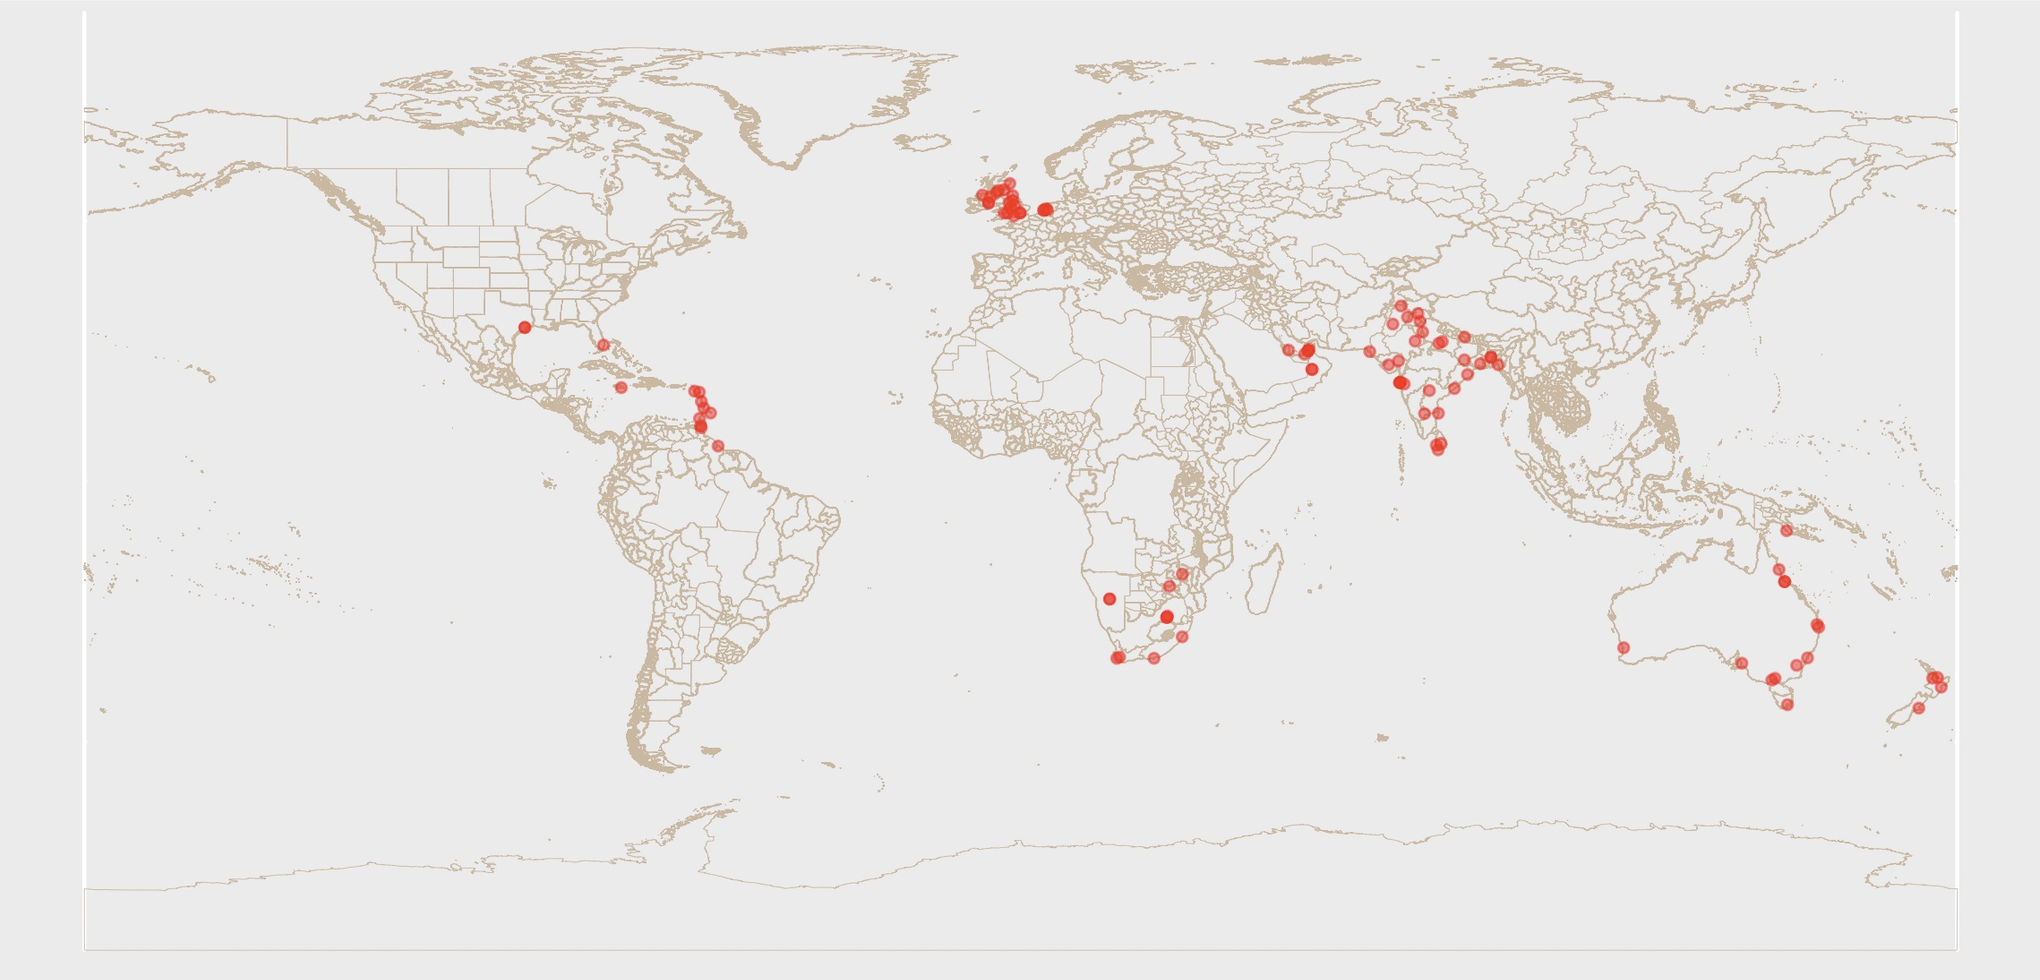
\includegraphics[width=1\linewidth]{~/OneDrive - UCB-O365/CricketCC/Code/cricket-climate/cricket-climate/venue-map}
\end{frame}

\begin{frame}{Identification}
\protect\hypertarget{identification}{}
Identification comes from variation in level of heat shock within and
across teams

Panel regression with fixed effects

$$
\begin{aligned}
y_{itmdv} &= \sum_{j} \beta_{j} TEMPSHOCK_{imdv} GAPBIN_{i} + \eta PRECIP_{mdv} + \nu HUMIDITY_{mdv}\\
& + \rho X_{mdv} + \theta_{t} + \theta_{order} + \theta_{type} + \theta_{innings} + \epsilon_{itmdv}
\end{aligned}
$$

\begin{itemize}
\tightlist
\item
  \(y_{itmdv}\) measure of productivity for player \(i\) in team \(t\)
  playing in match \(m\) on day \(d\) at venue \(v\)
\item
  \(\beta_{j}\) is the parameter of interest
\item
  \(TEMPSHOCK\) difference in temperature from previous game to current
\item
  \(GAPBIN\) gap in days between consecutive games
\item
  \(X_{mdv}\) aggregate opposing team's temperature shock
\item
  \(\theta_{t}\) team fixed effect
\item
  \(\theta_{order}\) batting order (only used for batsmen)
\item
  \(\theta_{type}\) game type - test, odi, t20, ipl
\end{itemize}
\end{frame}

\begin{frame}{Temperature Shock}
\protect\hypertarget{temperature-shock}{}
\tiny

\begin{longtable}[]{@{}
  >{\raggedright\arraybackslash}p{(\columnwidth - 8\tabcolsep) * \real{0.4079}}
  >{\centering\arraybackslash}p{(\columnwidth - 8\tabcolsep) * \real{0.1316}}
  >{\centering\arraybackslash}p{(\columnwidth - 8\tabcolsep) * \real{0.1447}}
  >{\centering\arraybackslash}p{(\columnwidth - 8\tabcolsep) * \real{0.1711}}
  >{\centering\arraybackslash}p{(\columnwidth - 8\tabcolsep) * \real{0.1447}}@{}}
\caption{Effect of temperature shocks on Batsmen
productivity}\tabularnewline
\toprule()
\begin{minipage}[b]{\linewidth}\raggedright
\end{minipage} & \begin{minipage}[b]{\linewidth}\centering
runs
\end{minipage} & \begin{minipage}[b]{\linewidth}\centering
balls
\end{minipage} & \begin{minipage}[b]{\linewidth}\centering
strike rate
\end{minipage} & \begin{minipage}[b]{\linewidth}\centering
boundary
\end{minipage} \\
\midrule()
\endfirsthead
\toprule()
\begin{minipage}[b]{\linewidth}\raggedright
\end{minipage} & \begin{minipage}[b]{\linewidth}\centering
runs
\end{minipage} & \begin{minipage}[b]{\linewidth}\centering
balls
\end{minipage} & \begin{minipage}[b]{\linewidth}\centering
strike rate
\end{minipage} & \begin{minipage}[b]{\linewidth}\centering
boundary
\end{minipage} \\
\midrule()
\endhead
interact\_var(-Inf,-2{]}.{[}0,3{]} & 2.1904 & 2.4082 & -0.9380 &
0.2894 \\
& (2.2576) & (2.0228) & (4.6905) & (0.3201) \\
interact\_var(2, Inf{]}.{[}0,3{]} & 0.3295 & 0.0535 & 3.9446 &
-0.0439 \\
& (2.0849) & (1.9167) & (6.1735) & (0.2427) \\
interact\_var(-Inf,-2{]}.(3,14{]} & 0.6498 & -0.5453 & 5.2349 &
0.1396 \\
& (1.5728) & (1.1517) & (4.6124) & (0.2240) \\
interact\_var(-2,2{]}.(3,14{]} & 4.3501** & 4.2370*** & 2.8813 &
0.5524** \\
& (1.3587) & (1.1911) & (3.5863) & (0.1895) \\
interact\_var(2, Inf{]}.(3,14{]} & 0.0535 & 0.0755 & -5.5751 & 0.1114 \\
& (1.6863) & (1.3342) & (4.0395) & (0.2304) \\
interact\_var(-Inf,-2{]}.(14,Inf{]} & 1.8042 & 1.9927+ & 0.6509 &
0.2565 \\
& (1.2252) & (1.0856) & (3.4026) & (0.1674) \\
interact\_var(-2,2{]}.(14,Inf{]} & 4.2559* & 5.4508** & -1.9252 &
0.4466+ \\
& (2.1053) & (2.0714) & (5.6913) & (0.2642) \\
interact\_var(2, Inf{]}.(14,Inf{]} & 2.4381+ & 2.2622* & 2.4666 &
0.3354+ \\
& (1.4056) & (1.1340) & (4.7113) & (0.1931) \\
precip & -0.1771* & -0.0667 & -0.6988** & -0.0341** \\
& (0.0841) & (0.0788) & (0.2640) & (0.0119) \\
humidity & 0.0644+ & 0.0363 & 0.0840 & 0.0095* \\
& (0.0354) & (0.0367) & (0.0901) & (0.0044) \\
opp\_team\_temp & 0.0782 & 0.0947 & -0.1370 & 0.0063 \\
& (0.0754) & (0.0673) & (0.2314) & (0.0100) \\
Num.Obs. & 2595 & 2595 & 2587 & 2595 \\
R2 & 0.107 & 0.106 & 0.017 & 0.107 \\
R2 Adj. & 0.099 & 0.098 & 0.008 & 0.099 \\
FE: batting\_order & X & X & X & X \\
FE: innings & X & X & X & X \\
\bottomrule()
\end{longtable}

\textbf{Note:} \^{}\^{} + p \textless{} 0.1, * p \textless{} 0.05, ** p
\textless{} 0.01, *** p \textless{} 0.001

Comparison : {[}-2,2{]}.{[}0,3{]}
\end{frame}

\begin{frame}{Temperature Shock}
\protect\hypertarget{temperature-shock-1}{}
\tiny

\begin{longtable}[]{@{}
  >{\raggedright\arraybackslash}p{(\columnwidth - 8\tabcolsep) * \real{0.4079}}
  >{\centering\arraybackslash}p{(\columnwidth - 8\tabcolsep) * \real{0.1447}}
  >{\centering\arraybackslash}p{(\columnwidth - 8\tabcolsep) * \real{0.1579}}
  >{\centering\arraybackslash}p{(\columnwidth - 8\tabcolsep) * \real{0.1316}}
  >{\centering\arraybackslash}p{(\columnwidth - 8\tabcolsep) * \real{0.1579}}@{}}
\caption{Effect of temperature shocks on Bowler's
productivity}\tabularnewline
\toprule()
\begin{minipage}[b]{\linewidth}\raggedright
\end{minipage} & \begin{minipage}[b]{\linewidth}\centering
economy
\end{minipage} & \begin{minipage}[b]{\linewidth}\centering
runs given
\end{minipage} & \begin{minipage}[b]{\linewidth}\centering
wicket
\end{minipage} & \begin{minipage}[b]{\linewidth}\centering
extras
\end{minipage} \\
\midrule()
\endfirsthead
\toprule()
\begin{minipage}[b]{\linewidth}\raggedright
\end{minipage} & \begin{minipage}[b]{\linewidth}\centering
economy
\end{minipage} & \begin{minipage}[b]{\linewidth}\centering
runs given
\end{minipage} & \begin{minipage}[b]{\linewidth}\centering
wicket
\end{minipage} & \begin{minipage}[b]{\linewidth}\centering
extras
\end{minipage} \\
\midrule()
\endhead
interact\_var(-Inf,-2{]}.{[}0,3{]} & -0.6979** & 2.9195+ & 0.1382 &
0.5684* \\
& (0.2579) & (1.5020) & (0.1571) & (0.2649) \\
interact\_var(2, Inf{]}.{[}0,3{]} & 0.2833 & 2.7649+ & 0.2796 &
0.3353 \\
& (0.4602) & (1.6610) & (0.2021) & (0.2762) \\
interact\_var(-Inf,-2{]}.(3,14{]} & 0.2700 & -0.2136 & -0.2569* &
0.1798 \\
& (0.3019) & (1.2531) & (0.1202) & (0.1772) \\
interact\_var(-2,2{]}.(3,14{]} & -0.2454 & 3.5985*** & -0.0484 &
0.1600 \\
& (0.2169) & (0.9288) & (0.0808) & (0.1567) \\
interact\_var(2, Inf{]}.(3,14{]} & -0.0126 & 0.9541 & 0.0258 &
-0.0064 \\
& (0.2275) & (0.9492) & (0.1169) & (0.1560) \\
interact\_var(-Inf,-2{]}.(14,Inf{]} & 0.0050 & 3.1747** & -0.0325 &
0.2261 \\
& (0.1768) & (0.9660) & (0.0786) & (0.1586) \\
interact\_var(-2,2{]}.(14,Inf{]} & -0.0724 & 6.6789*** & -0.1830 &
0.5746* \\
& (0.2481) & (1.7958) & (0.1206) & (0.2257) \\
interact\_var(2, Inf{]}.(14,Inf{]} & 0.0089 & 3.0158** & 0.0903 &
0.3558* \\
& (0.2131) & (1.1303) & (0.1111) & (0.1605) \\
precip & -0.0185 & -0.1918** & -0.0001 & -0.0263*** \\
& (0.0212) & (0.0719) & (0.0052) & (0.0076) \\
humidity & 0.0008 & 0.0617** & -0.0013 & 0.0071+ \\
& (0.0055) & (0.0210) & (0.0020) & (0.0041) \\
opp\_team\_temp & -0.0183 & 0.0666 & -0.0017 & 0.0065 \\
& (0.0126) & (0.0614) & (0.0059) & (0.0103) \\
Num.Obs. & 1734 & 1734 & 1734 & 1734 \\
R2 & 0.079 & 0.057 & 0.026 & 0.038 \\
R2 Adj. & 0.058 & 0.036 & 0.005 & 0.016 \\
FE: bowling\_team & X & X & X & X \\
FE: innings & X & X & X & X \\
\bottomrule()
\end{longtable}

\textbf{Note:} \^{}\^{} + p \textless{} 0.1, * p \textless{} 0.05, ** p
\textless{} 0.01, *** p \textless{} 0.001

Comparison : {[}-2,2{]}.{[}0,3{]}
\end{frame}

\begin{frame}{Heat Accumulation}
\protect\hypertarget{heat-accumulation}{}
\tiny

\begin{longtable}[]{@{}
  >{\raggedright\arraybackslash}p{(\columnwidth - 8\tabcolsep) * \real{0.4211}}
  >{\centering\arraybackslash}p{(\columnwidth - 8\tabcolsep) * \real{0.1316}}
  >{\centering\arraybackslash}p{(\columnwidth - 8\tabcolsep) * \real{0.1316}}
  >{\centering\arraybackslash}p{(\columnwidth - 8\tabcolsep) * \real{0.1711}}
  >{\centering\arraybackslash}p{(\columnwidth - 8\tabcolsep) * \real{0.1447}}@{}}
\caption{Effect of heat accumulation on Batsmen
productivity}\tabularnewline
\toprule()
\begin{minipage}[b]{\linewidth}\raggedright
\end{minipage} & \begin{minipage}[b]{\linewidth}\centering
runs
\end{minipage} & \begin{minipage}[b]{\linewidth}\centering
balls
\end{minipage} & \begin{minipage}[b]{\linewidth}\centering
strike rate
\end{minipage} & \begin{minipage}[b]{\linewidth}\centering
boundary
\end{minipage} \\
\midrule()
\endfirsthead
\toprule()
\begin{minipage}[b]{\linewidth}\raggedright
\end{minipage} & \begin{minipage}[b]{\linewidth}\centering
runs
\end{minipage} & \begin{minipage}[b]{\linewidth}\centering
balls
\end{minipage} & \begin{minipage}[b]{\linewidth}\centering
strike rate
\end{minipage} & \begin{minipage}[b]{\linewidth}\centering
boundary
\end{minipage} \\
\midrule()
\endhead
interact\_home{[}0,100{]}.{[}0,3{]} & -2.5550 & -1.8530 & -0.4230 &
-0.3733 \\
& (2.0909) & (1.7497) & (4.7965) & (0.2766) \\
interact\_home(100,Inf{]}.{[}0,3{]} & -2.9127+ & -2.8080* & -0.4361 &
-0.3711 \\
& (1.5564) & (1.0998) & (3.9255) & (0.2300) \\
interact\_home{[}0,100{]}.(3,14{]} & -2.1182 & -0.8958 & -5.5853 &
-0.2766 \\
& (1.8272) & (1.5643) & (3.9690) & (0.2431) \\
interact\_home{[}0,100{]}.(14,Inf{]} & -0.9679 & 0.0939 & -2.4776 &
-0.1644 \\
& (2.0234) & (1.7029) & (4.8759) & (0.2618) \\
interact\_home(100,Inf{]}.(14,Inf{]} & -1.3547 & -1.0155 & 1.2014 &
-0.1577 \\
& (1.9953) & (1.5580) & (5.4900) & (0.2769) \\
precip & -0.2010* & -0.0862 & -0.7732** & -0.0367** \\
& (0.0889) & (0.0795) & (0.2903) & (0.0125) \\
humidity & 0.0731* & 0.0568+ & 0.0562 & 0.0092+ \\
& (0.0357) & (0.0321) & (0.1022) & (0.0047) \\
opp\_team\_temp & 0.0702 & 0.1133+ & -0.2850 & 0.0043 \\
& (0.0711) & (0.0614) & (0.2051) & (0.0094) \\
Num.Obs. & 2595 & 2595 & 2587 & 2595 \\
R2 & 0.111 & 0.122 & 0.054 & 0.116 \\
R2 Adj. & 0.095 & 0.107 & 0.037 & 0.101 \\
FE: batting\_team & X & X & X & X \\
FE: batting\_order & X & X & X & X \\
FE: innings & X & X & X & X \\
\bottomrule()
\end{longtable}

\textbf{Note:} \^{}\^{} + p \textless{} 0.1, * p \textless{} 0.05, ** p
\textless{} 0.01, *** p \textless{} 0.001

;Comparison : {[}0,50{]}.{[}0,3{]}
\end{frame}

\begin{frame}{Heat Accumulation}
\protect\hypertarget{heat-accumulation-1}{}
\tiny

\begin{longtable}[]{@{}
  >{\raggedright\arraybackslash}p{(\columnwidth - 8\tabcolsep) * \real{0.4211}}
  >{\centering\arraybackslash}p{(\columnwidth - 8\tabcolsep) * \real{0.1316}}
  >{\centering\arraybackslash}p{(\columnwidth - 8\tabcolsep) * \real{0.1579}}
  >{\centering\arraybackslash}p{(\columnwidth - 8\tabcolsep) * \real{0.1316}}
  >{\centering\arraybackslash}p{(\columnwidth - 8\tabcolsep) * \real{0.1579}}@{}}
\caption{Effect of heat accumulation on Bowler's
productivity}\tabularnewline
\toprule()
\begin{minipage}[b]{\linewidth}\raggedright
\end{minipage} & \begin{minipage}[b]{\linewidth}\centering
economy
\end{minipage} & \begin{minipage}[b]{\linewidth}\centering
runs given
\end{minipage} & \begin{minipage}[b]{\linewidth}\centering
wicket
\end{minipage} & \begin{minipage}[b]{\linewidth}\centering
extras
\end{minipage} \\
\midrule()
\endfirsthead
\toprule()
\begin{minipage}[b]{\linewidth}\raggedright
\end{minipage} & \begin{minipage}[b]{\linewidth}\centering
economy
\end{minipage} & \begin{minipage}[b]{\linewidth}\centering
runs given
\end{minipage} & \begin{minipage}[b]{\linewidth}\centering
wicket
\end{minipage} & \begin{minipage}[b]{\linewidth}\centering
extras
\end{minipage} \\
\midrule()
\endhead
interact\_home{[}0,100{]}.{[}0,3{]} & -0.2554 & -0.7013 & 0.2114+ &
0.1364 \\
& (0.2409) & (1.3661) & (0.1183) & (0.1781) \\
interact\_home(100,Inf{]}.{[}0,3{]} & -0.2633 & -2.1149* & 0.1752+ &
-0.1354 \\
& (0.2012) & (1.0088) & (0.0973) & (0.1594) \\
interact\_home{[}0,100{]}.(3,14{]} & -0.4879* & -0.7530 & 0.1280 &
-0.0261 \\
& (0.2418) & (1.3050) & (0.1210) & (0.1771) \\
interact\_home{[}0,100{]}.(14,Inf{]} & -0.2197 & 1.0770 & 0.1039 &
0.1952 \\
& (0.2026) & (1.4172) & (0.1175) & (0.1667) \\
interact\_home(100,Inf{]}.(14,Inf{]} & -0.1792 & 2.1235+ & 0.1858+ &
0.2148 \\
& (0.2433) & (1.2172) & (0.1105) & (0.1796) \\
precip & -0.0178 & -0.1905* & -0.0005 & -0.0285*** \\
& (0.0217) & (0.0738) & (0.0052) & (0.0075) \\
humidity & 0.0007 & 0.0647** & -0.0015 & 0.0073+ \\
& (0.0055) & (0.0221) & (0.0020) & (0.0041) \\
opp\_team\_temp & -0.0163 & 0.0829 & 0.0034 & 0.0059 \\
& (0.0098) & (0.0501) & (0.0052) & (0.0102) \\
Num.Obs. & 1734 & 1734 & 1734 & 1734 \\
R2 & 0.076 & 0.048 & 0.022 & 0.034 \\
R2 Adj. & 0.057 & 0.028 & 0.002 & 0.014 \\
FE: bowling\_team & X & X & X & X \\
FE: innings & X & X & X & X \\
\bottomrule()
\end{longtable}

\textbf{Note:} \^{}\^{} + p \textless{} 0.1, * p \textless{} 0.05, ** p
\textless{} 0.01, *** p \textless{} 0.001

;Comparison : {[}0,50{]}.{[}0,3{]}
\end{frame}

\begin{frame}{Excessive Heat - Batsmen}
\protect\hypertarget{excessive-heat---batsmen}{}
\tiny

\begin{longtable}[]{@{}
  >{\raggedright\arraybackslash}p{(\columnwidth - 8\tabcolsep) * \real{0.3472}}
  >{\centering\arraybackslash}p{(\columnwidth - 8\tabcolsep) * \real{0.1528}}
  >{\centering\arraybackslash}p{(\columnwidth - 8\tabcolsep) * \real{0.1528}}
  >{\centering\arraybackslash}p{(\columnwidth - 8\tabcolsep) * \real{0.1806}}
  >{\centering\arraybackslash}p{(\columnwidth - 8\tabcolsep) * \real{0.1667}}@{}}
\caption{Effect of excessive heat on Batsmen
productivity}\tabularnewline
\toprule()
\begin{minipage}[b]{\linewidth}\raggedright
\end{minipage} & \begin{minipage}[b]{\linewidth}\centering
runs
\end{minipage} & \begin{minipage}[b]{\linewidth}\centering
balls
\end{minipage} & \begin{minipage}[b]{\linewidth}\centering
strike rate
\end{minipage} & \begin{minipage}[b]{\linewidth}\centering
boundary
\end{minipage} \\
\midrule()
\endfirsthead
\toprule()
\begin{minipage}[b]{\linewidth}\raggedright
\end{minipage} & \begin{minipage}[b]{\linewidth}\centering
runs
\end{minipage} & \begin{minipage}[b]{\linewidth}\centering
balls
\end{minipage} & \begin{minipage}[b]{\linewidth}\centering
strike rate
\end{minipage} & \begin{minipage}[b]{\linewidth}\centering
boundary
\end{minipage} \\
\midrule()
\endhead
interact\_shock0.{[}0,3{]} & -1.2526 & -0.4638 & -0.9734 & -0.1902 \\
& (1.4970) & (1.2321) & (4.0287) & (0.1947) \\
interact\_shock1.{[}0,3{]} & 2.7785 & 2.9229+ & 6.6888 & 0.2454 \\
& (1.8986) & (1.6061) & (5.5123) & (0.2463) \\
interact\_shock0.(3,14{]} & -1.3290 & -0.7044 & 0.3060 & -0.1727 \\
& (1.6662) & (1.4076) & (4.8812) & (0.2114) \\
interact\_shock1.(3,14{]} & 4.4439* & 5.1743*** & 0.9382 & 0.4876* \\
& (1.8555) & (1.5274) & (5.5627) & (0.2414) \\
interact\_shock1.(14,Inf{]} & 4.0523* & 5.3086** & 3.8688 & 0.4074+ \\
& (1.8683) & (1.5839) & (5.8581) & (0.2374) \\
precip & -0.2563** & -0.1357+ & -0.8466** & -0.0429*** \\
& (0.0856) & (0.0746) & (0.2907) & (0.0124) \\
humidity & 0.1059** & 0.0921** & 0.0909 & 0.0127** \\
& (0.0368) & (0.0327) & (0.1111) & (0.0048) \\
opp\_team\_temp & -0.0552 & -0.0172 & -0.4023+ & -0.0094 \\
& (0.0796) & (0.0718) & (0.2272) & (0.0101) \\
Num.Obs. & 2595 & 2595 & 2587 & 2595 \\
R2 & 0.115 & 0.130 & 0.054 & 0.119 \\
R2 Adj. & 0.100 & 0.115 & 0.037 & 0.104 \\
FE: batting\_team & X & X & X & X \\
FE: batting\_order & X & X & X & X \\
FE: innings & X & X & X & X \\
\bottomrule()
\end{longtable}

\textbf{Note:} \^{}\^{} + p \textless{} 0.1, * p \textless{} 0.05, ** p
\textless{} 0.01, *** p \textless{} 0.001
\end{frame}

\begin{frame}{Excessive Heat - Bowler}
\protect\hypertarget{excessive-heat---bowler}{}
\tiny

\begin{longtable}[]{@{}
  >{\raggedright\arraybackslash}p{(\columnwidth - 8\tabcolsep) * \real{0.3623}}
  >{\centering\arraybackslash}p{(\columnwidth - 8\tabcolsep) * \real{0.1449}}
  >{\centering\arraybackslash}p{(\columnwidth - 8\tabcolsep) * \real{0.1739}}
  >{\centering\arraybackslash}p{(\columnwidth - 8\tabcolsep) * \real{0.1449}}
  >{\centering\arraybackslash}p{(\columnwidth - 8\tabcolsep) * \real{0.1739}}@{}}
\caption{Effect of excessive heat on Bowler's
productivity}\tabularnewline
\toprule()
\begin{minipage}[b]{\linewidth}\raggedright
\end{minipage} & \begin{minipage}[b]{\linewidth}\centering
economy
\end{minipage} & \begin{minipage}[b]{\linewidth}\centering
runs given
\end{minipage} & \begin{minipage}[b]{\linewidth}\centering
wicket
\end{minipage} & \begin{minipage}[b]{\linewidth}\centering
extras
\end{minipage} \\
\midrule()
\endfirsthead
\toprule()
\begin{minipage}[b]{\linewidth}\raggedright
\end{minipage} & \begin{minipage}[b]{\linewidth}\centering
economy
\end{minipage} & \begin{minipage}[b]{\linewidth}\centering
runs given
\end{minipage} & \begin{minipage}[b]{\linewidth}\centering
wicket
\end{minipage} & \begin{minipage}[b]{\linewidth}\centering
extras
\end{minipage} \\
\midrule()
\endhead
interact\_shock0.{[}0,3{]} & -0.0976 & -4.4859*** & 0.0037 & -0.1890 \\
& (0.2143) & (1.1125) & (0.0983) & (0.1962) \\
interact\_shock1.{[}0,3{]} & -0.2564 & -0.6354 & -0.1287 & -0.1483 \\
& (0.2579) & (1.5145) & (0.1275) & (0.2242) \\
interact\_shock0.(3,14{]} & -0.1522 & -4.4082*** & -0.1281 & -0.0160 \\
& (0.2777) & (1.1770) & (0.1159) & (0.2358) \\
interact\_shock1.(3,14{]} & -0.1638 & 0.4652 & -0.2382* & -0.2421 \\
& (0.2430) & (1.5948) & (0.1142) & (0.2163) \\
interact\_shock1.(14,Inf{]} & -0.1805 & 0.9016 & -0.1809 & 0.0723 \\
& (0.2161) & (1.5591) & (0.1147) & (0.2383) \\
precip & -0.0170 & -0.2356** & 0.0012 & -0.0279*** \\
& (0.0213) & (0.0725) & (0.0053) & (0.0078) \\
humidity & -0.0005 & 0.0854*** & -0.0027 & 0.0072+ \\
& (0.0054) & (0.0235) & (0.0021) & (0.0042) \\
opp\_team\_temp & -0.0135 & 0.0047 & 0.0080 & 0.0060 \\
& (0.0105) & (0.0577) & (0.0058) & (0.0121) \\
Num.Obs. & 1734 & 1734 & 1734 & 1734 \\
R2 & 0.074 & 0.057 & 0.023 & 0.033 \\
R2 Adj. & 0.055 & 0.038 & 0.003 & 0.013 \\
FE: bowling\_team & X & X & X & X \\
FE: innings & X & X & X & X \\
\bottomrule()
\end{longtable}

\textbf{Note:} \^{}\^{} + p \textless{} 0.1, * p \textless{} 0.05, ** p
\textless{} 0.01, *** p \textless{} 0.001
\end{frame}

\begin{frame}{Next Steps}
\protect\hypertarget{next-steps}{}
\begin{enumerate}
\tightlist
\item
  More on incentives
\end{enumerate}

\begin{itemize}
\tightlist
\item
  International games vs League games
\item
  Presence of Supertars \textcolor{brown}{[Brown 2011]}
\end{itemize}

\begin{enumerate}
\setcounter{enumi}{1}
\item
  Why are batsmen \& bowlers behaving differently?
\item
  Heat accumulation measure by month and not aggregate
\end{enumerate}
\end{frame}

\begin{frame}{End}
\protect\hypertarget{end}{}
\[
\text{Thank you!}
\]
\end{frame}

\end{document}
